\section{ResNet-LDDMM, or LDDMM revisited}
\label{sec:ResNet-LDDMM}

The central idea in our ResNet-LDDMM is to make use of a particular family of deep neural networks, i.e. residual deep networks (or ResNets), to solve the flow equation Eq. (\ref{Eq:LDDMM}). In supervised learning, a residual network \cite{DBLP:conf/cvpr/HeZRS16,DBLP:conf/eccv/HeZRS16} has the following form:

\begin{equation}
h^{l+1} = h^{l} + f^{l}(h^{l},\theta^{l})    
\label{Eq:hidden}
\end{equation}

\noindent where $h^{l}$ is the trainable hidden layer, $l\in \{1,\dots,L\}$, and $\theta^l\in \{\theta^1,\dots,\theta^L\}$ denotes the network parameters. Compared to a standard feed-forward network, where $h^{l+1} = f(h^{l},\theta^{l})$, at the heart of ResNet is the ultimate idea that every additional layer should contain the identity function as one of its elements. Thus, a residual $h^{l+1}-h^{l}$ is learned instead of transforming the output of the previous layer $h^{l}$ to $h^{l+1}$. Recent works have pointed out a striking similarity between this important property in residual networks and the numerical solution of ordinary differential equations (e.g. \cite{weinan2017proposal,haber2017stable,ruthotto2020machine}) using the forward Euler method with a given initial value. In fact, training a deep residual network is viewed as a discretization of a dynamical training system governed by a first-order ODE, where the network layers are viewed as time-steps and the network parameters $\theta^l$ are interpreted as the \textit{control} to optimize \cite{liu2019deep}. %In particular, ResNet can be seen as an \textit{Euler discretization} of a first-order ODE. 

\begin{figure*}[ht]
  \centering
   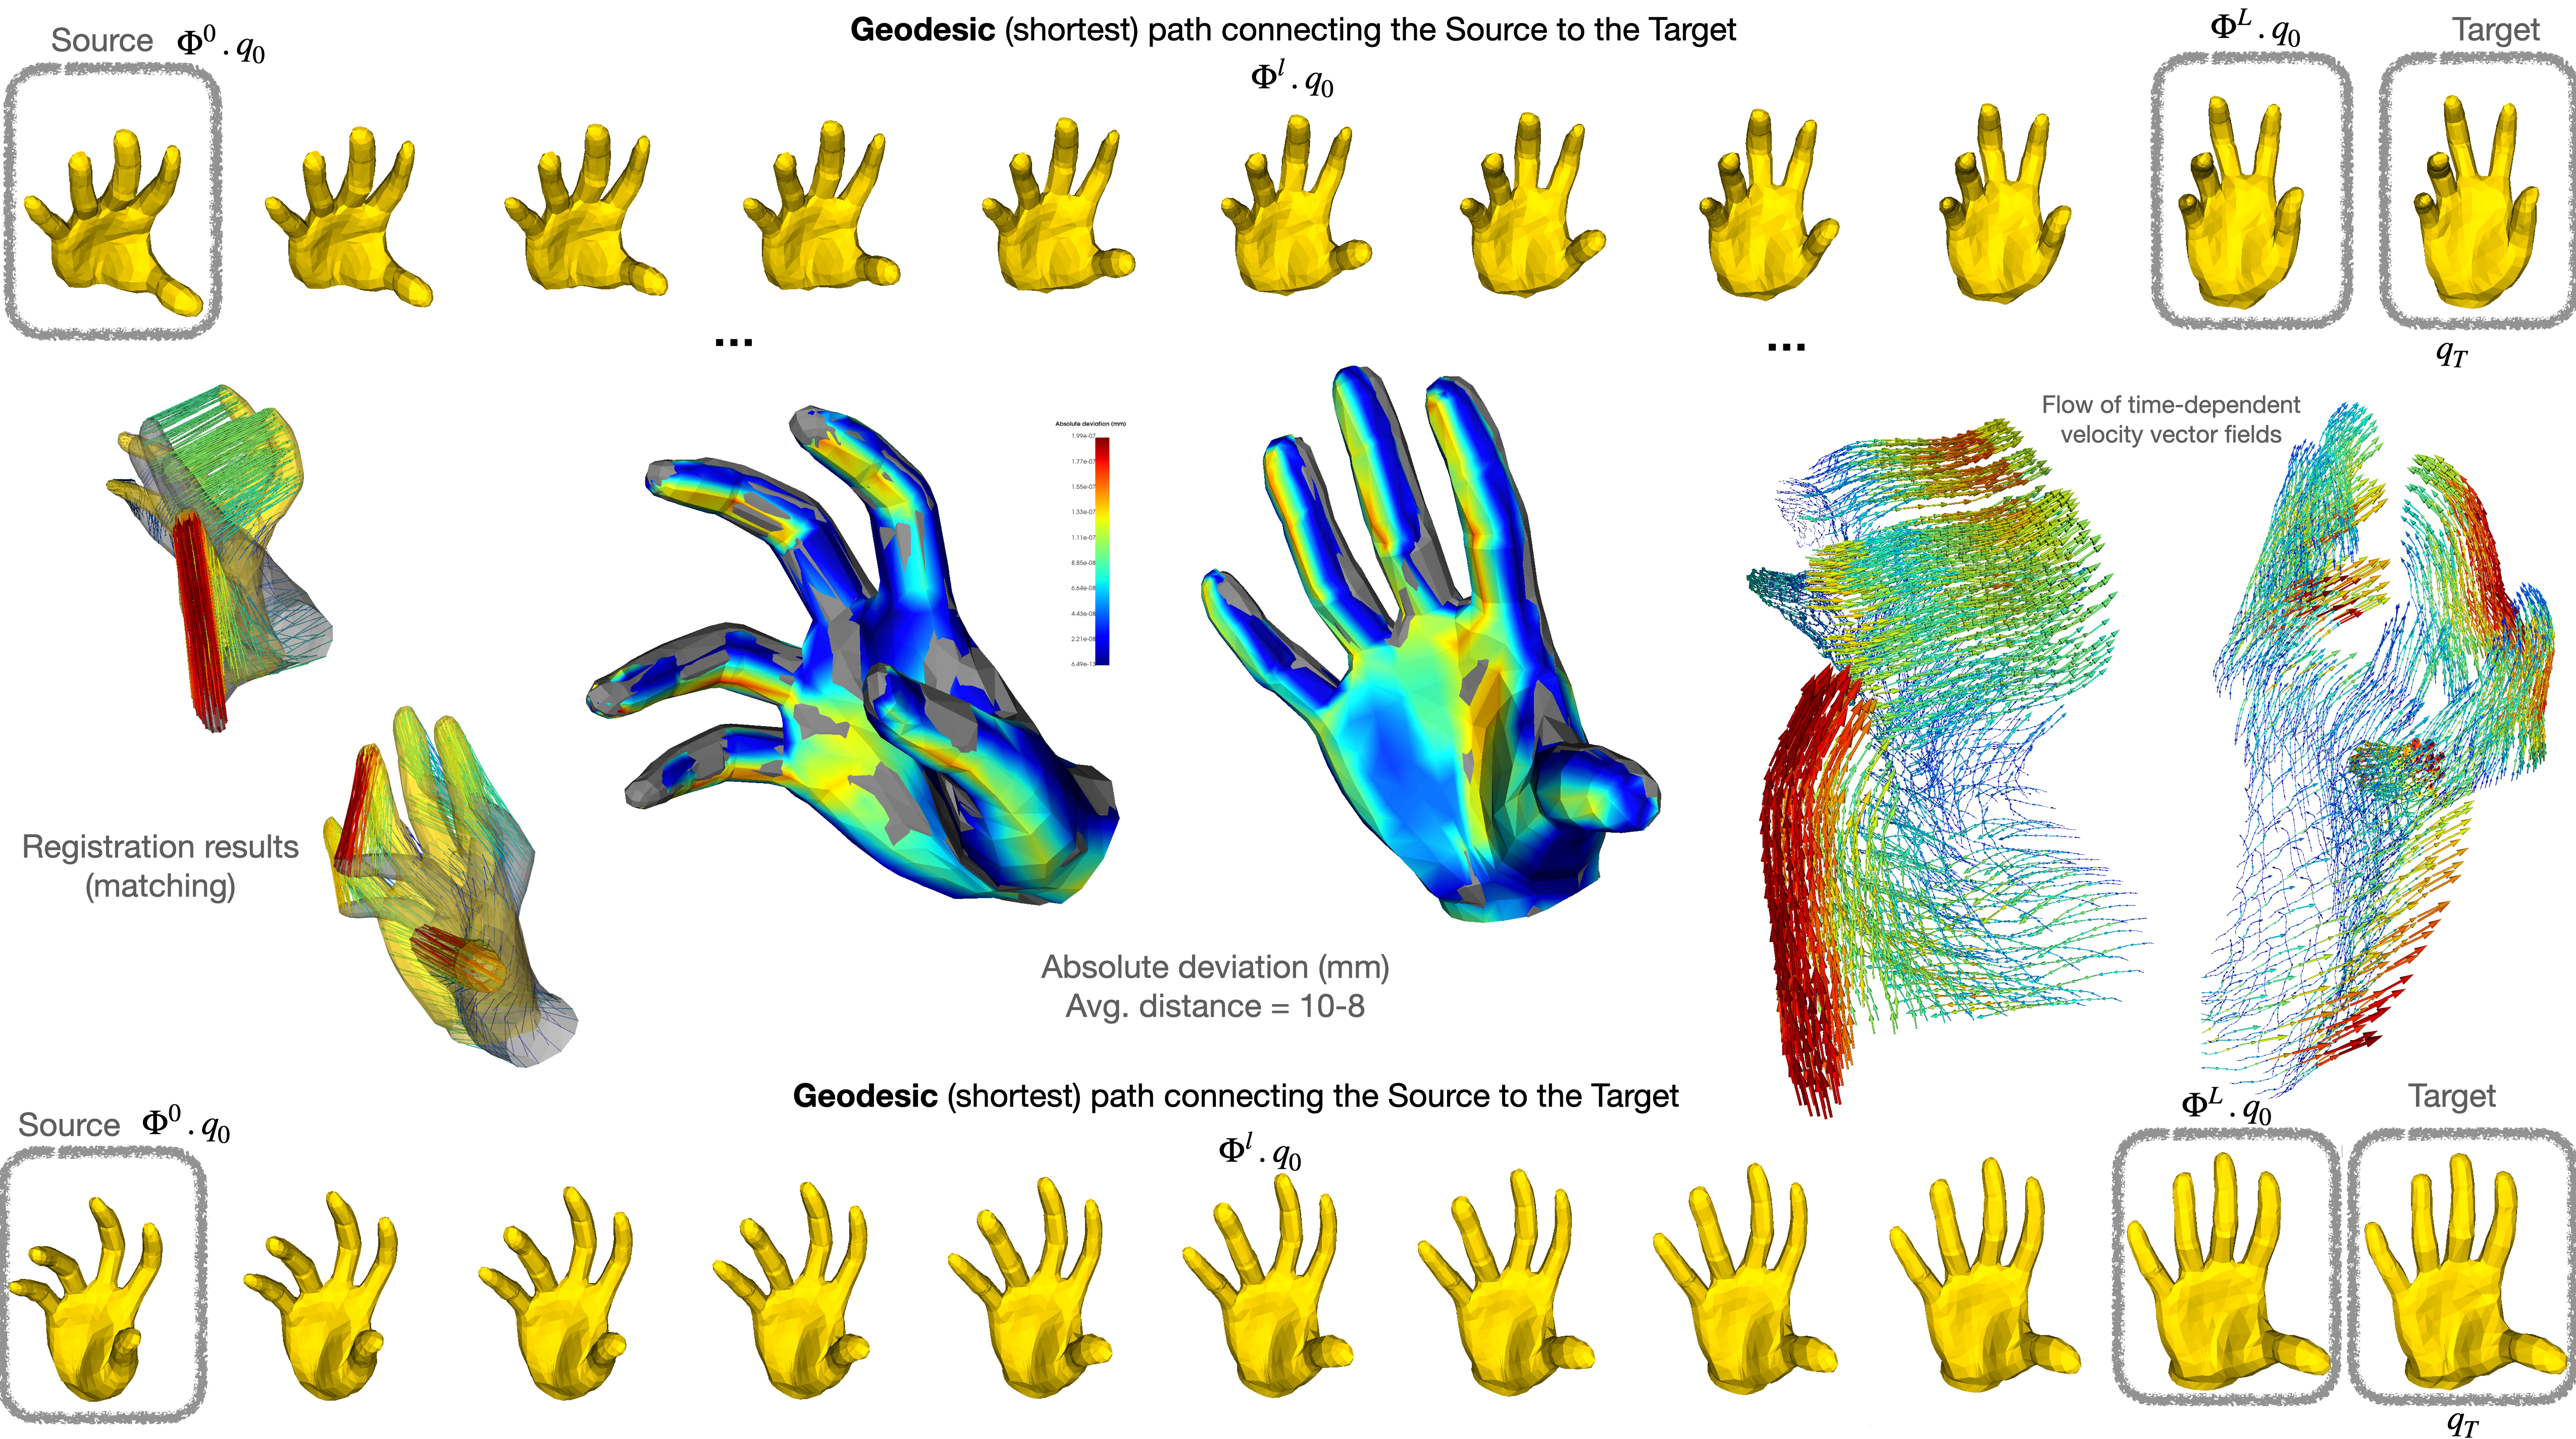
\includegraphics[width=\linewidth]{Figs/Hands_FirstExample.png}
  \vspace{-0.5cm}
  \caption{A pictorial summary of our diffeomorphic registration results. Top: a geodesic path connecting a source hand shape to a target shape; Bottom: the inverse path (source and target change roles); Center-right: both flows of the time-dependent velocity fields $f^l(.,\theta^l)$, building blocks of our ResNet-LDDMM. Center-left: final Euclidean displacements and registration results.}
   \label{Fig:Example}
\end{figure*}

Inspired by the general formulation and aiming to solve the flow equation Eq. (\ref{Eq:FlowEq}), we build our ResNet-LDDMM framework. As shown in Fig. \ref{Fig:Overview}, our ResNet-LDDMM is an ensemble of $L$ successive identical building blocks. Each building block is composed of three fully connected layers and a point-wise ReLU activation function separating the first two layers. From the LDDMM perspective (right panel of Fig. \ref{Fig:Overview}), each building block ${f^l}$ represents a velocity vector field $\real^3\rightarrow\real^3$ at a discrete time $l$. The $f^l$ are   parameterized by $\theta^l$. If $f^l$ are sufficiently smooth and spatially regular (we postpone this demonstration to Sec. \ref{sec:Diffeos}), one can then build a diffeomorphic transformation $\Phi^f(1)$ (by integration of Eq. (\ref{Eq:ResNet})) that moves the initial shape $q_S$ to fit $q_T$, which is mathematically equivalent to $\Phi(1).q_S \sim q_T$ and  $\Phi(1)=\Phi^L$:

\begin{equation}
\Phi^{l+1}.q_0 = \Phi^{l}.q_0 + \Delta^L f^l(\Phi^{l}.q_0,\theta^{l}),\ \text{with}\ \Delta^L=\frac{1}{L}.
\label{Eq:ResNet}
\end{equation}

Compared to the conventional LDDMM formulation, here, the time-varying velocity vector fields are deep neural networks $f^l(.,\theta^l)$ that should be optimized with respect to a fit error. To this end and if assume a ResNet-LDDMM with number of blocks $L \to \infty$ (i.e. $\frac{1}{L}\to 0$), we cast Eq. (\ref{Eq:LDDMM}) as,  
%Consequently, find a minimizer $v^*$ (and the corresponding flow $\Phi^v(1,.)$) turns to find the best weights $\Theta^*=\{\theta^0,\dots,\theta^L\}$ of the network which minimizes Eq.(\ref{Eq:FlowEq}) and subject of a regularization term on $v$, or equivalently on functions $f(.,\theta^l)$, $l\in{0,\dots,L}$. If assuming a Network with number of building blocks $\to \infty$ (i.e. $\frac{1}{L}\to 0$), Eq.(\ref{Eq:LDDMM}) becomes,
\begin{equation}
\begin{split}
\Theta^*, \Phi^*(1)=\argmin_{\Theta=\{\theta^t\}_{t \in [0,1]}}\frac{1}{2\sigma^2}\mathcal{D}(\Phi^{\Theta}(1).q_S,q_{T})\\
+\frac{1}{2} \int_{0}^{1}  \| f^t(\Phi^{\Theta}(t).q_S,\theta^{t}) \|_{\ell^2}^2 dt, %+ \lambda \int_{0}^{1}\|\theta^{l}\|^2_{2} dl
\end{split}
\label{Eq:ResNet-LDDMM}
\end{equation}

\noindent subject to $\partial_t \Phi^{\Theta}(t,.)=f^t(\Phi^{\Theta}(t,.),\theta^{t})$ for a.e. $t \in [0, 1]$ and $\Phi(0,.)$ denotes the identity map (the neutral element of the group $\textrm{Diff}(\real^3)$). The family $f^t(.,\theta^t)$ is the ensemble of functions to be approximated by the network which coincides with the time-dependent velocity fields along the time interval $[0,1]$ and $\Theta=(\theta^t)_{t \in [0,1]}$ are the whole ResNet-LDDMM parameters. $\Phi^{\Theta}(1)$ is the final transformation and $\Phi^{\Theta}(t)$ are the intermediate transformations. The choice of ${\cal D}(.,.)$ will be detailed in the next paragraph. The second term is a regularizer that presents the length of the path connecting $q_S$ to $\Phi^{\Theta}(t).q_S$, on the orbit of $q_S$, which ensures that the optimal vector field stays regular enough to ensure topology preserving transformations (Sec. \ref{sec:GeometricRegularization}). In the right panel of Fig. \ref{Fig:Overview} we illustrate how ResNet-LDDMM enables a minimizing path (a geodesic) on the orbit of $q_s$. Intermediate shapes are discrete elements of the geodesic outputs of the action of the intermediate diffeomorphisms $\Phi^l$ on the source shape $q_S$. $\Phi^l$ are deduced from the optimal vector fields $f^l(.,\theta^l)$ sitting in between the panels of Fig. \ref{Fig:Overview} (colors (cold $\to$ hot) reflect the absolute amount of displacement at each time-step and at a vertex-level).

% \subsection{ResNet-LDDMM Network Architecture}
% \label{sec:Architecture}

\textbf{ResNet-LDDMM Network Architecture.} Let us now come back to the architecture of our ResNet-LDDMM. As illustrated in the left panel of Fig. \ref{Fig:Overview}, our network takes as inputs (1) the source shape $q_S$, or to be more accurate $\Phi^{0}.q_S$, where $\Phi^{0}$ is the identity diffeomorphism of $\real^3$, and (2) an initial guess $\Theta_0=(\theta_0^1,\dots,\theta_0^l)$, initial parameters of the network and (3) the target shape $q_T$ to evaluate the loss function Eq. (\ref{Eq:ResNet-LDDMM}). The \textit{velocity fields} $f^{l}(\cdot,\theta^l)$ and the corresponding diffeomorphisms $\Phi^{l}$ are predicted by the $l$-indexed successive building blocks of the network (orange box in Fig. \ref{Fig:Overview}). The number of building blocks $L$ in the ResNet-LDDMM coincides with the total number of time-steps in the conventional LDDMM, once discretized. 

-- Each \textbf{building block} (denoted by $f^l(.,\theta^l)$ and generating the $l$-th velocity field on $\real^3$) consists of three successive fully connected weight layers. Weight matrices $W_i$ and bias vectors $b_i$ (limited to the first and second weight layers) define point-wise convolution operations, with kernel filters of size $1\times 1(\times m)$, performed separately on all points. This is equivalent to designing a fully connected layer as described in the Network-in-Network \cite{lin2014network}. We will denote $m$ as the width of individual building blocks. Subsequently, a ReLU activation function is applied to the output of the first weight layer within each building block. The last weight layer reduces the dimensionality of the output of the previous layer to get velocity vectors in $\real^3$ (so, the width of this layer is exactly $3$).  While the weight layers conduct affine transformations of the input (output of the previous building block), ReLU reduces to zeros all negative outputs of the first layer, thus dividing the space $\real^3$ into $m$-half spaces for more flexible prediction of the velocity fields (this point will be detailed in Sec. \ref{sec:GeometricDescription}). 

-- The \textbf{identity map}, which connects successive building blocks of our ResNet-LDDMM allows the network to focus predicting the difference $\Phi^l-\Phi^{l-1}$, and thus time-dependent velocity fields. This specific architecture allows a forward Euler scheme to solve the non-stationary ODE (flow equation Eq. (\ref{Eq:FlowEq})). Intuitively, an individual building block $f^l$ will move each point $x^l\in q^l$ into $x^{l+1}\in q^{l+1}$ such that passing the three successive connected layers results in

\begin{equation}
\begin{split}
x^{l+1}-x^l=&f^l(x^l,\theta^l).\Delta^L
\\=& W^l_3(W^l_2(ReLU(W^l_1x^l+b^l_1)+b^l_2).\Delta^L
\end{split}
\end{equation}

\noindent Here $W^l_i$ are the set of filters and $b^l_i$ biases which compose the weight layers.% and ReLU is an element-wise activation function. 

-- The \textbf{loss function} ${\cal J}(\Theta$) given in Eq. (\ref{Eq:ResNet-LDDMM}) to be minimized consists of a data term and the integration of instantaneous kinetic energy terms as a regularization term. While the data term pushes the deformed template $\Phi^{L}.q_S$ closer to the target $q_T$ by minimizing an appropriate distance between point clouds, the regularization controls activities of the building blocks, i.e. their outputs. These terms are balanced with the $1/2\sigma^2$ parameter, as defined in Eq. (\ref{Eq:ResNet-LDDMM}).

-- As a \textbf{data attachment} term, we use either a point-wise distance called the \textit{Chamfer's distance (CD)} (Eq. (\ref{Eq:Chamfer})) or a global distance measure referred to us the \textit{Earth mover’s distance (EMD)}, the \textit{Wasserstein distance} or the \textit{Optimal Transport (OT) costs} (Eq. (\ref{Eq:Wasserstein})). The former measures the squared distance between each point in one set to its nearest neighbor in the other set and vice verse. Mathematically, it is formulated as follows: Eq. (\ref{Eq:Chamfer}),

\begin{equation}
    {\cal D^{CD}}(q_1,q_2)=\sum_{x\in q_1} \min_{y \in q_2} \|x-y\|^2_2 + \sum_{x\in q_2}\min_{y \in q_1} \|x-y\|^2_2.
\label{Eq:Chamfer}    
\end{equation}


The second distance first introduced in \cite{rubner2000earth}, measures the discrepancy between distributions when accounting for their respective geometries \cite{feydy2019interpolating}, defined by Eq. (\ref{Eq:Wasserstein}):



\begin{equation}
{\cal D^{EMD}}(q_1,q_2)=\min_{\xi}\sum_{(x,y)\in q_1\times q_2} \|x-y\|^p_2\xi(x,y).
\label{Eq:Wasserstein}    
\end{equation}



\noindent The \textit{Earth Mover's distance} ${\cal D^{EMD}}$ corresponds to $p=1$ and is based on finding a transport plan $\xi: q_1\times q_2\rightarrow [0,1]$, such that $\sum_{x\in q_1} \xi(x,y^*)=\frac{1}{n_2}$ and $\sum_{y\in q_2} \xi(x^*,y)=\frac{1}{n_1}$ for all $x^*$ in $q_1$ and $y^*$ in $q_2$, with $n_1$ and $n_2$ respectively the number of points in $q_1$ and $q_2$. The function $\xi(x,y)$ represents the proportion of mass at $x$ that is transported to $y$. One can also take $p=2$ instead, which corresponds to the \textit{Wasserstein} distance.
%It solves an optimization problem as in Eq. (\ref{Eq:Wasserstein}). 
In practice, the iterative \textit{Sinkhorn’s Algorithm} is used to approximate the EMD distance, i.e. an Optimal Transport with Entropic Constraints (the reader is directed to \cite{NIPS2013_af21d0c9} and \cite{chizat2020faster} for more details). Importantly, we note that both distances are differentiable almost everywhere \cite{feydy2017optimal}. The choice of distance used in the data term depends on the data itself and the nature of the deformations, as we will discuss in Sec. \ref{sec:Experiments}.   
%\footnote{https://github.com/jaberkow/TensorFlowSinkhorn}
\begin{figure}[ht]
  \centering
  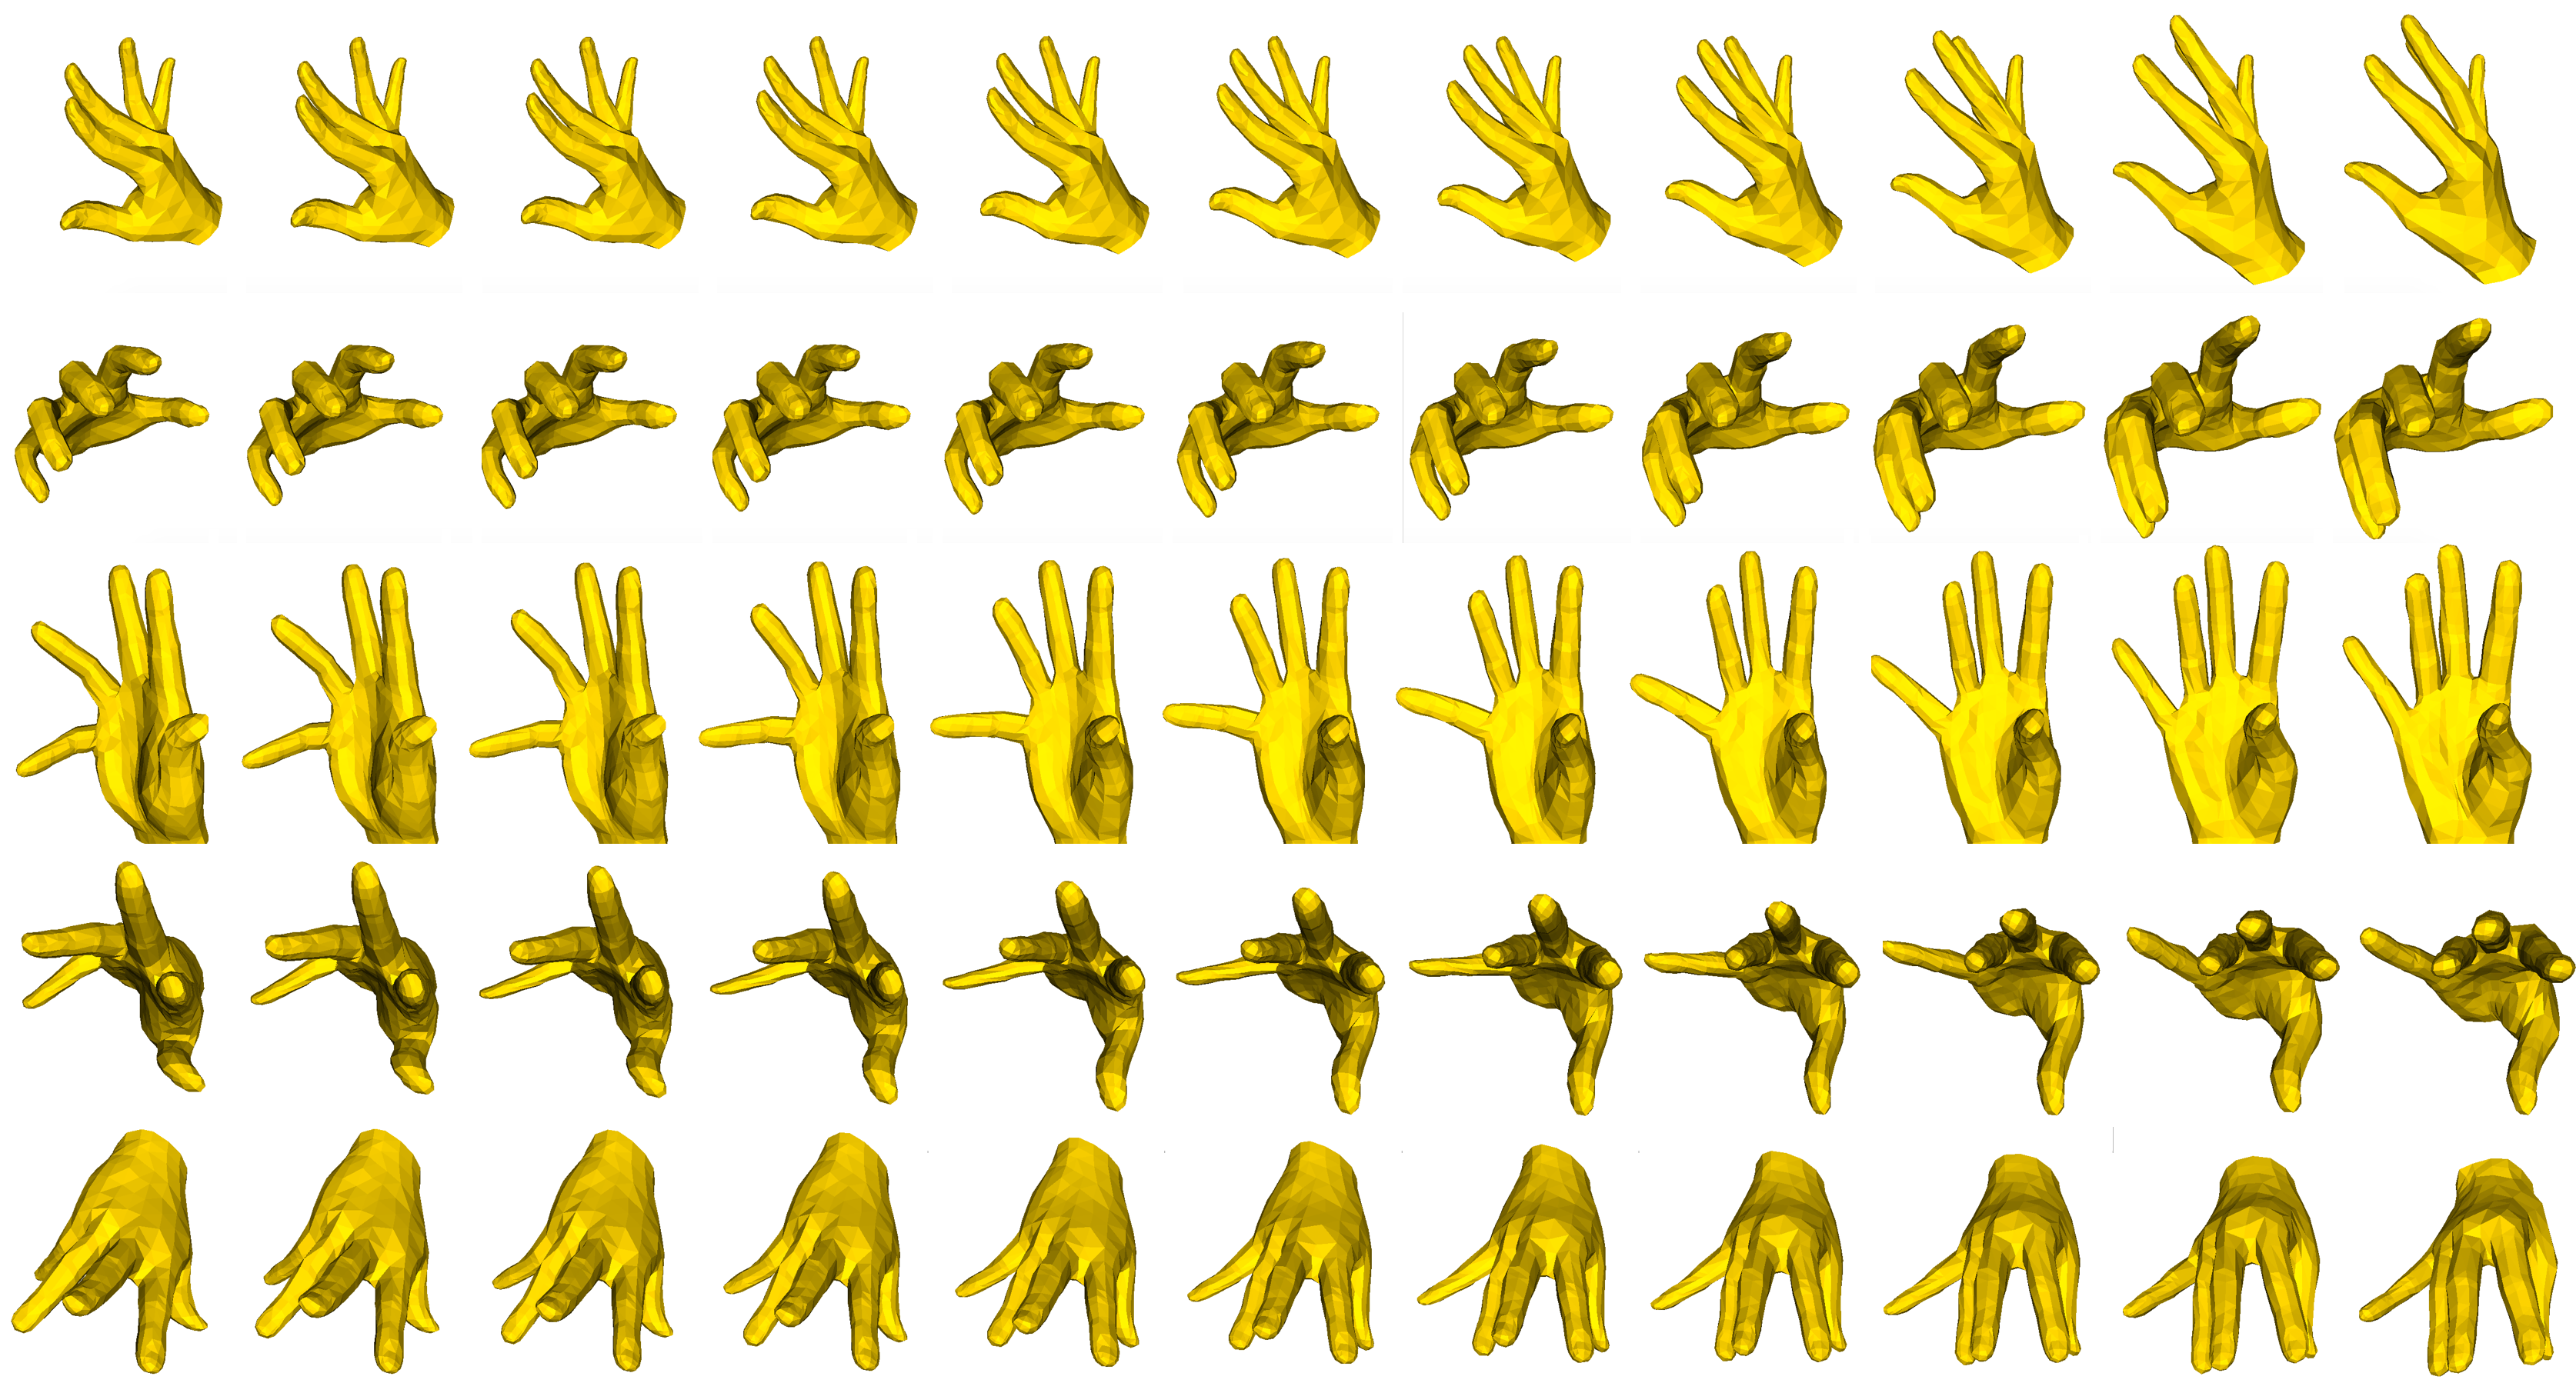
\includegraphics[width=\linewidth]{Figs/Hands2.png}
   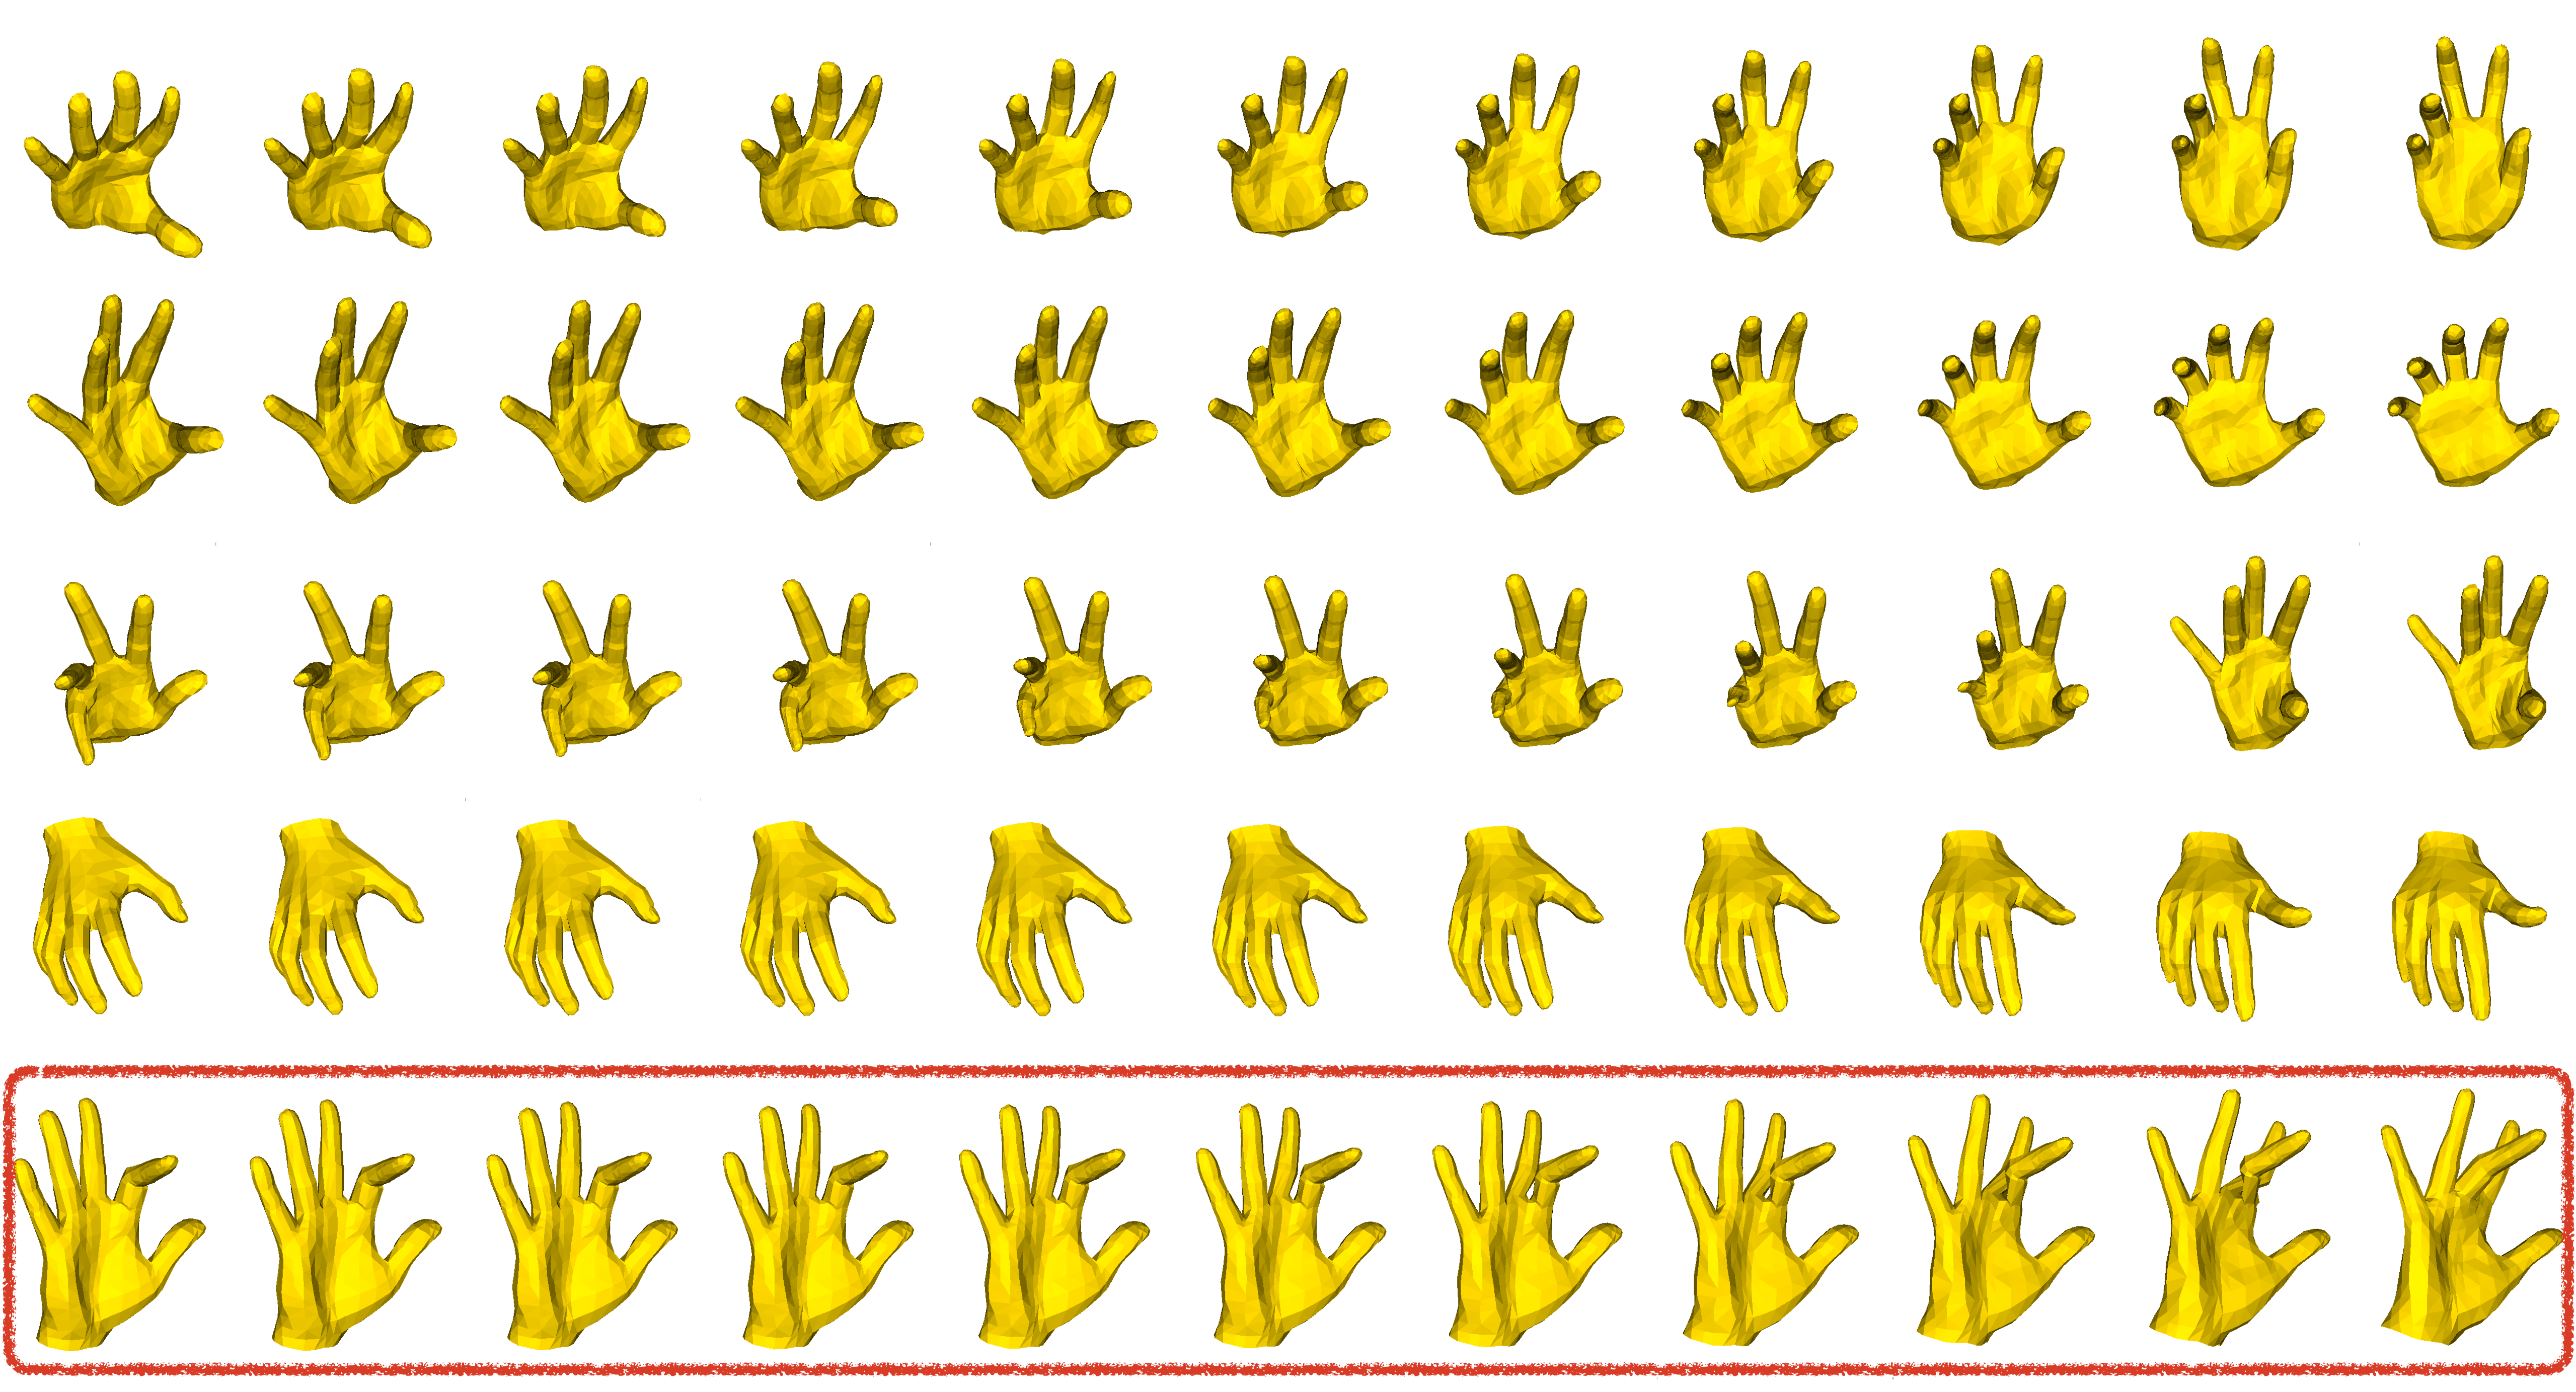
\includegraphics[width=\linewidth]{Figs/HandsExamples.png}
   \vspace{-0.8cm}
  \caption{Geodesic paths connecting source (left) and target (right) hand shapes modulo deformations. Last row provides and example of a wrong transformation (index and middle fingers interchanged).}
   \label{Fig:ExampleHands}
\end{figure}

-- Following LDDMM algorithms (e.g. \cite{younes2009evolutions} and \cite{miller2006geodesic}), our \textbf{regularizer} is a summation over all kinetic energies of the system at all time-steps ${\cal S}(f)=\frac{1}{2}\int_0^1 {\cal S}_t(f^t) dt$, where, ${\cal S}_t(f)=\| f^t(\Phi^{\Theta}(t,.),\theta^{t}) \|_{\ell_2}^2$. The main difference is that while LDDMM makes use of the $\|.\|_{\cal A}$ of the RKHS induced by Gaussian Kernel $K$ with a fixed deformation scale, our ResNet-LDDMM uses the $\|.\|_{\ell_2}$ on the neural functions $f^l(.,\theta^l)$. Consequently, ResNet-LDDMM generates geodesics by minimizing the amount of energy spent to get close to $q_T$ from $q_S$, when traveling along the Orbit of $q_S$. We summarize the steps of our algorithm ResNet-LDDMM in Algo. \ref{Algo:ResNet-LDDMM}.    

\begin{algorithm}
\caption{ResNet-LDDMM.}
\begin{algorithmic}%[1]
\REQUIRE Source shape $q_{S}$, Target shape $q_{T}$, $L$: \# of blocks, $\eta$: learning rate, $\Delta^L = 1/L$: time-step, E:\# of iter., $m$: ResNet's width (\# of filters), $\sigma$ (see Eq. (\ref{Eq:ResNet-LDDMM})) .  
 \STATE $ l \leftarrow 1$, $e \leftarrow 0$, $\Phi^0=I_{\real^3}$
 \STATE Set $ \Theta=\{\theta^l\}_{l \in {1..L}} \leftarrow \Theta_0$ (initial guess)
 \STATE Set $q^{0} \leftarrow \Phi^0.q_S$ (initial state)
% \STATE $\tilde{\Phi^0}(q^0) \leftarrow FC(q^{0},m)$ (dim. expansion)
 \WHILE{$e<E$ (epoch)} 
  \WHILE{$l<L$ (building block)} 
  \STATE Compute $v^{l} \leftarrow f^{l}(\Phi^{l-1}.q^{l-1},\theta^{l})\Delta^L$
  %\STATE Compute $v^l \leftarrow g(\tilde{v}^l,\theta^{l},3)$ (dim. reduction)
  \STATE Update $\Phi^{l} \leftarrow \Phi^{l-1} + v^{l}$ %f^{l}(\Phi^{l-1}.q^{l-1},\theta^{l})\Delta^L$ 
  \ENDWHILE
  \STATE Compute $q^{L}\leftarrow q^0+\sum_{l=1}^{L} v^l$ ($\Phi^{L}\leftarrow \Phi^0+\sum_{l=1}^{L} v^l$)
  \STATE Evaluate the loss function $\mathcal{J}(\Theta^{e})$ (Eq. (\ref{Eq:ResNet-LDDMM})) at epoch $e$
  \STATE Update $\Theta_{e+1} \leftarrow \Theta_{e} - \eta \nabla_{\Theta} \mathcal{J}(\Theta)$ %\frac{\partial \mathcal{J}}{\partial \Theta}$
\ENDWHILE
\STATE Compute $\Theta^*$ minimizer of Eq. (\ref{Eq:ResNet-LDDMM}) using ADAM.
   \ENSURE $\Phi^*(.,1) \leftarrow \Phi^{L}$ parameterized by $\Theta^*$: final transformation; $\{f^l\}_l$: flow of velocity fields.
 \end{algorithmic} 
\label{Algo:ResNet-LDDMM}
\end{algorithm}

We show in Fig. \ref{Fig:Example} both paths from a source shape (on the left) and a target shape (on the right). We illustrate the flows of velocity fields obtained for $L=10$ intermediate time-steps. We can see also how close are the deformed sources to the target shapes (from the absolute spatial deviations). The examples involving hands, shown in Fig. \ref{Fig:ExampleHands}, are particularly interesting (because of the nature of deformations possible for the hand) and challenging at the same time (as different neighboring fingers can exhibit opposite movements). The last example, depicted in a red box, shows a case where ResNet-LDDMM fails in matching corresponding fingers. In fact, while the transformation is a diffeomorphism (by swapping the index and middle fingers), an incorrect registration result is obtained. Algo. \ref{Algo:GeometricFramework} summarizes the steps for building a geodesic path connecting a source shape to a target shape using the output transformations of Algo. \ref{Algo:ResNet-LDDMM}. Note that here we make use of the EMD distance $\cal D^{EMD}$ as data attachment term, more suitable to compare articulated shapes than the \textit{Chamfer's distance}.

\begin{algorithm}
\caption{Optimal Trajectory on the \textit{Orbit} of $q_S$.}
\begin{algorithmic}[1]
\REQUIRE Source shape $q_{S}$; Target shape $q_{T}$; $\sigma$ (Eq. (\ref{Eq:ResNet-LDDMM})).
\STATE $l \leftarrow 1$ 
\STATE Compute $\Phi(1)$, $\{f^l\}_l$ using Algo. \ref{Algo:ResNet-LDDMM}.
\WHILE{$l\leq L$}
  \STATE Compute $\dot{q}^{l} \leftarrow f^{l}(.,\theta^l)$ ($\dot{q}^{l} \in T_{q^l}([q_S])$: the instantaneous shape's speed, $[q_S]$: Shape Space)
  \STATE Update the shape $q^{l+1} \leftarrow q^{l} + \dot{q}^{l}$ (on $\cal S$)
  \ENDWHILE
\ENSURE Discrete steps $q^{l}$, ${l\in\{1,\dots,L\}}$ of an optimal trajectory connecting $q^{0} \leftarrow q_S$ to $q^{L}\sim q_T$.
\end{algorithmic} 
\label{Algo:GeometricFramework}
\end{algorithm}

\begin{figure*}[ht!]
  \centering
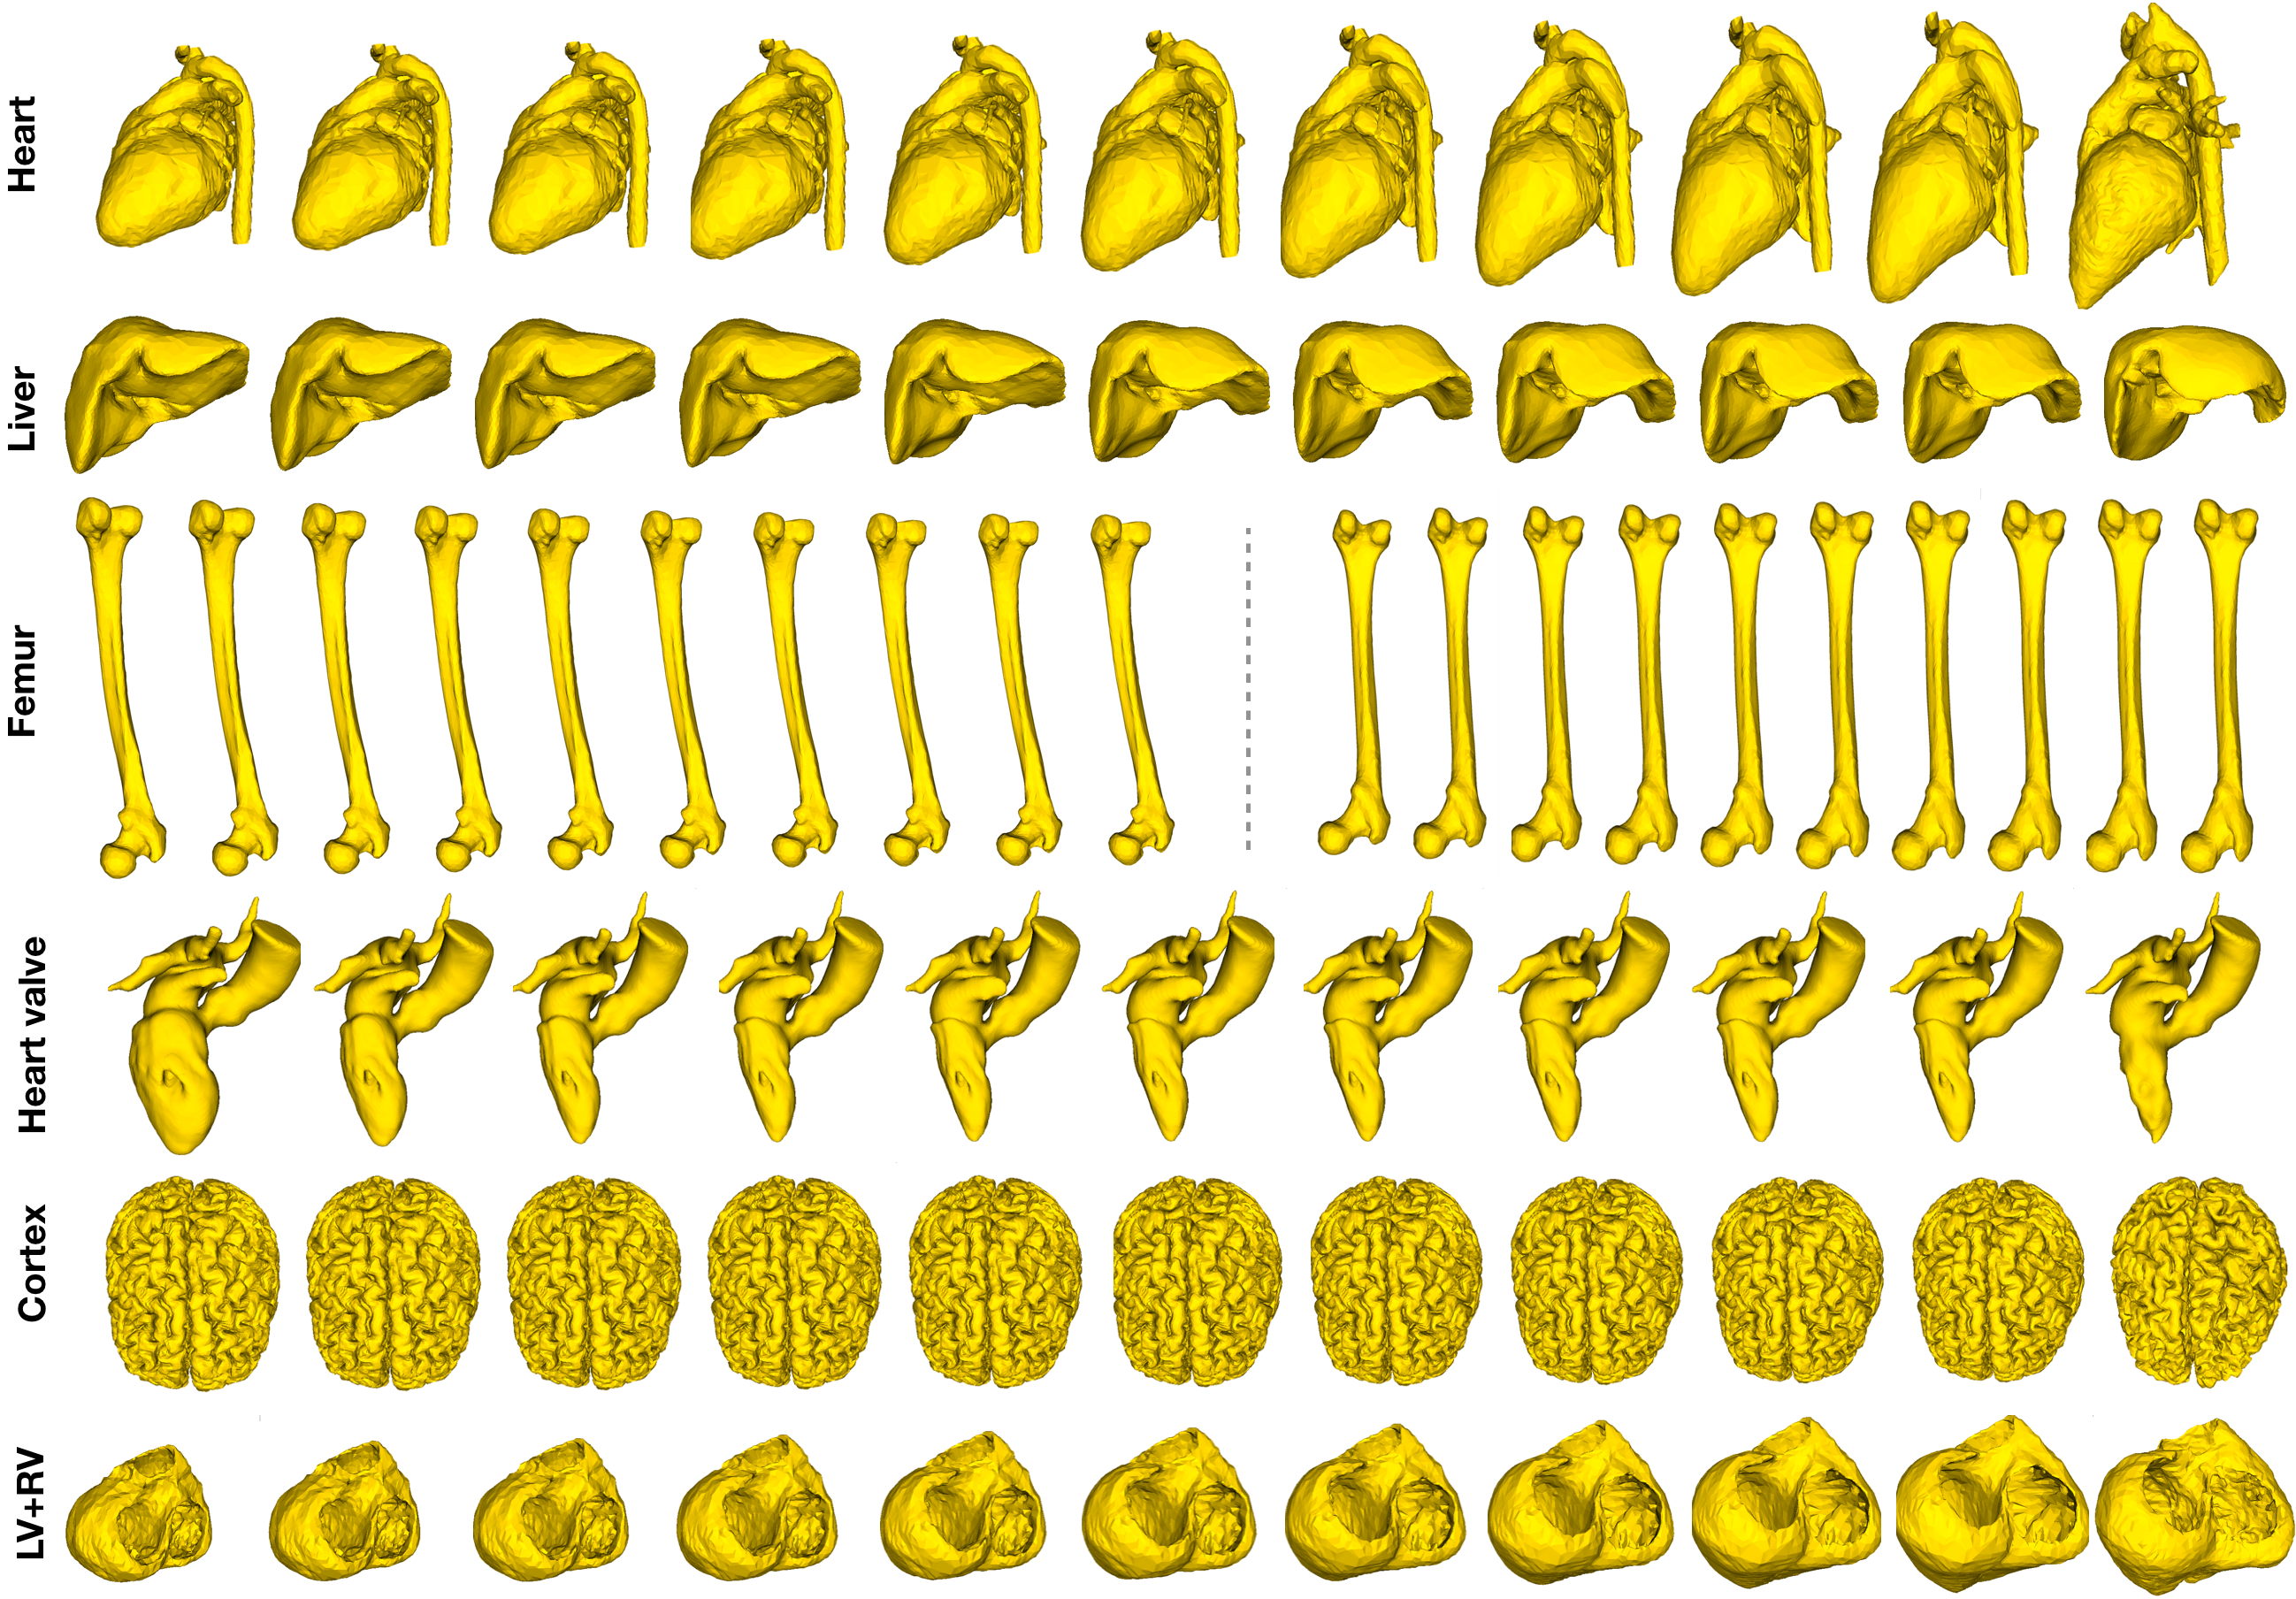
\includegraphics[width=\linewidth]{Figs/Anatomy.png}
    \vspace{-0.5cm}
  \caption{Geodesic paths connecting source (first column) and target anatomical shapes (last column) of different subjects. From top to bottom: whole heart, liver, femur 1-to-2 (left) followed by femur 2-to-1 (right), heart valve, cortex and LV+RV (left and right ventricles of pathological hearts).}
   \label{Fig:CAExamples}
\end{figure*}

To demonstrate the performance of ResNet-LDDMM in registering anatomical parts of the human body, we provide in Fig. \ref{Fig:CAExamples} several examples of optimal deformations. Shapes are 3D triangulated surfaces obtained from manual segmentation of MRI images of different subjects. Note that here the $\cal D^{CD}$ distance is used to compute the data attachment term in Eq.(\ref{Eq:ResNet-LDDMM}). In each row, we show the source shape on the left, the target shape on the right and discrete steps from the geodesic path connecting them, except for the femur example, where both paths from the source to the target and inversely, are reported. %Fig.\ref{Fig:Valves} show registration details between heart valves.  



